% Foliensatz: "AFu-Kurs nach DJ4UF" von DK0TU, Amateurfunkgruppe der TU Berlin
% Lizenz: CC BY-NC-SA 3.0 de (http://creativecommons.org/licenses/by-nc-sa/3.0/de/)
% Autoren: Felix Baum <baum@campus.tu-berlin.de>
% Korrekturen: Lars Weiler <dc4lw@darc.de>

\documentclass[aspectratio=169]{beamer}

\usepackage[ngerman]{babel} % deutsche Worttrennung etc.
\usepackage[utf8]{inputenc} % UTF8 Text

\usepackage[super, comma, numbers, square, sort]{natbib}

\usepackage{hyperref}       % Hyperref Package für bessere Referenzen (todo)
\hypersetup{
	colorlinks=false,       %   false: boxed links; true: colored links
    %linkcolor=white,       %   color of internal links (change box color with linkbordercolor)
    citecolor=red,          %   color of links to bibliography
    filecolor=white,        %   color of file links
    urlcolor=blue           %   color of external links
}

\usepackage{multirow}
\usepackage{wasysym}  % Math Symbols like \permil
%\usepackage{colortbl}
%\usepackage{subscript}
%\usepackage{caption}
%\usepackage{setspace}
%\usepackage{xcolor}        % benutze CodeListe

% Footnote
%\usepackage{hanging}
%
%\setbeamertemplate{footnote}{%
%  \hangpara{2em}{1}%
%  \makebox[2em][l]{\insertfootnotemark}\footnotesize\insertfootnotetext\par%
%}


%\usepackage{pgf}
%\usepackage{tikz}
%\usetikzlibrary{arrows,automata}
%\usetikzlibrary{positioning}
%
%\tikzset{
%    state/.style={
%           rectangle,
%           rounded corners,
%           draw=black, very thick,
%           minimum height=2em,
%           minimum width=2pt,
%           inner sep=2pt,
%           text centered,
%           },
%}

%\usepackage{listings}
%\lstset{basicstyle=\small, numberstyle=\tiny, extendedchars=true, numbers=left, numbersep=5pt}
%\lstset{showtabs=false, showspaces=false, showstringspaces=false}
%%\lstset{backgroundcolor=\color{white!75!lightgray}, , frame=single}
%%\lstset{backgroundcolor=\color{white}}
%%\lstset{backgroundcolor=none}
%\lstset{keywordstyle=\color{blue!50!gray},  identifierstyle=\color{black}}
%\lstset{commentstyle=\color{green!50!gray}, stringstyle=\color{red!50!gray}}
%\lstset{language=C, fontadjust=true, tabsize=2, breaklines=true}
%\lstset{backgroundcolor=\color{white!75!lightgray}, caption=\lstname, frame=single}
%\lstset{emphstyle=\color{black}\fbox}
%
%% Keine "Listing:"-Caption
%\captionsetup{labelformat=empty,labelsep=none}
%
%% für mathematische Umgebungen
%\usepackage{amsmath,amsfonts,amssymb}
%
%\lstdefinestyle{Bash}{
%language=Bash,
%frame=single,
%rulecolor=\color{black},
%backgroundcolor=\color{gray!50},
%keywordstyle=\color{black},
%identifierstyle=,
%commentstyle=\color{black},
%stringstyle=\color{magenta!65!white},
%showstringspaces=false,
%basicstyle=\footnotesize\ttfamily\color{black},
%numbers=none,
%breaklines=true,
%captionpos=b
%}

%\usepackage{listings}
%
%\lstdefinestyle{basic}{
%    captionpos=t,%
%    basicstyle=\footnotesize\ttfamily,%
%    numberstyle=\tiny,%
%    numbers=left,%
%    stepnumber=1,%
%    frame=single,%
%    showspaces=false,%
%    showstringspaces=false,%
%    showtabs=false,%
%    %
%    keywordstyle=\color{blue},%
%    identifierstyle=,%
%    commentstyle=\color{gray},%
%    stringstyle=\color{magenta}%
%}



% fließende Boxen haben keinen Abstand
%\fboxsep0mm

% inkludiere Creative Commons Helper
%%%%%%%%%%%%%%%%%%%%%%%%%%%%%%%%%%%%%%%%%%%%%%%%%%%%%%%%%%%%%%%%
%% ccBeamer 0.1, 2007-07-02                                   %%
%% Written by Sebastian Pipping <webmaster@hartwork.org>      %%
%% ---------------------------------------------------------- %%
%% Licensed under Creative Commons Attribution-ShareAlike 3.0 %%
%% http://creativecommons.org/licenses/by-sa/3.0/             %%
%%%%%%%%%%%%%%%%%%%%%%%%%%%%%%%%%%%%%%%%%%%%%%%%%%%%%%%%%%%%%%%%


%% Images
\newcommand{\CcImageBy}[1]{%
	
\includegraphics[scale=#1]{texdata/creative_commons/cc_by_30.pdf}%
}
\newcommand{\CcImageCc}[1]{%
	
\includegraphics[scale=#1]{texdata/creative_commons/cc_cc_30.pdf}%
}
\newcommand{\CcImageDevNations}[1]{%
	
\includegraphics[scale=#1]{texdata/creative_commons/cc_dev_nations_30.pdf}%
}
\newcommand{\CcImageNc}[1]{%
	
\includegraphics[scale=#1]{texdata/creative_commons/cc_nc_30.pdf}%
}
\newcommand{\CcImageNd}[1]{%
	
\includegraphics[scale=#1]{texdata/creative_commons/cc_nd_30.pdf}%
}
\newcommand{\CcImagePd}[1]{%
	
\includegraphics[scale=#1]{texdata/creative_commons/cc_pd_30.pdf}%
}
\newcommand{\CcImageSa}[1]{%
	
\includegraphics[scale=#1]{texdata/creative_commons/cc_sa_30.pdf}%
}
\newcommand{\CcImageSampling}[1]{%
	
\includegraphics[scale=#1]{texdata/creative_commons/cc_sampling_30.pdf}%
}
\newcommand{\CcImageSamplingPlus}[1]{%
	
\includegraphics[scale=#1]{texdata/creative_commons/cc_sampling_plus_30.pdf}%
}


%% Groups
\newcommand{\CcGroupBy}[2]{% zoom, gap
	\CcImageCc{#1}\hspace*{#2}\CcImageBy{#1}%
}
\newcommand{\CcGroupByNc}[2]{% zoom, gap
	\CcImageCc{#1}\hspace*{#2}\CcImageBy{#1}\hspace*{#2}\CcImageNc{#1}%
}
\newcommand{\CcGroupByNcNd}[2]{% zoom, gap
	\CcImageCc{#1}\hspace*{#2}\CcImageBy{#1}\hspace*{#2}\CcImageNc{#1}\hspace*{#2}\CcImageNd{#1}%
}
\newcommand{\CcGroupByNcSa}[2]{% zoom, gap
	\CcImageCc{#1}\hspace*{#2}\CcImageBy{#1}\hspace*{#2}\CcImageNc{#1}\hspace*{#2}\CcImageSa{#1}%
}
\newcommand{\CcGroupByNd}[2]{% zoom, gap
	\CcImageCc{#1}\hspace*{#2}\CcImageBy{#1}\hspace*{#2}\CcImageNd{#1}%
}
\newcommand{\CcGroupBySa}[2]{% zoom, gap
	\CcImageCc{#1}\hspace*{#2}\CcImageBy{#1}\hspace*{#2}\CcImageSa{#1}%
}
\newcommand{\CcGroupDevNations}[2]{% zoom, gap
	\CcImageCc{#1}\hspace*{#2}\CcImageDevNations{#1}%
}
\newcommand{\CcGroupNcSampling}[2]{% zoom, gap
	\CcImageCc{#1}\hspace*{#2}\CcImageNc{#1}\hspace*{#2}\CcImageSampling{#1}%
}
\newcommand{\CcGroupPd}[1]{% zoom
	\CcImagePd{#1}%
}
\newcommand{\CcGroupSampling}[1]{% zoom
	\CcImageSampling{#1}%
}
\newcommand{\CcGroupSamplingPlus}[1]{% zoom
	\CcImageSamplingPlus{#1}%
}


%% Text
\newcommand{\CcLongnameBy}{Attribution}
\newcommand{\CcLongnameByNc}{Attribution-NonCommercial}
\newcommand{\CcLongnameByNcNd}{Attribution-NoDerivs}
\newcommand{\CcLongnameByNcSa}{Attribution-NonCommercial-ShareAlike}
\newcommand{\CcLongnameByNd}{Attribution-NoDerivs}
\newcommand{\CcLongnameBySa}{Attribution-ShareAlike}

\newcommand{\CcNote}[1]{% longname
	This work is licensed under the \textit{Creative Commons #1 3.0 License}.%
}


% generelles Thema auswählen
\usetheme{Goettingen} %Berlin spart ohne Sidebar allerdings angenehm Platz
% AnnArbor | Antibes | Bergen | Berkeley | Berlin | Boadilla | boxes | CambridgeUS | Copenhagen | Darmstadt | default | Dresden | Frankfurt | Goettingen | Hannover | Ilmenau | JuanLesPins | Luebeck | Madrid | Malmoe | Marburg | Montpellier | PaloAlto | Pittsburgh | Rochester | Singapore | Szeged | Warsaw

% Farben wählen
\usecolortheme{beetle}
% beaver | beetle | crane | default | dolphin | dove | fly | lily | orchid | rose | seagull | seahorse | sidebartab | structure | whale | wolverine

% Setze alle Farben auf Grau und Weiß
%\definecolor{craneorange}{RGB}{64,64,64}
%\definecolor{craneblue}{RGB}{255,255,255}

% Schriftart wählen
\usefonttheme{default}
% default | professionalfonts | serif | structurebold | structureitalicserif | structuresmallcapsserif

% Innere Themen(Kopf-, Fuß-, Sidebar usw)
%\useinnertheme{default}
\useinnertheme{circles}
% default | inmargin | rectangles | rounded | circles

% Äußere Themen (Anordnung der inneren, grenzen der Folien etc.)
\useoutertheme{infolines}
% default | infolines | miniframes | shadow | sidebar | smoothbars | smoothtree | split | tree

% Deaktiviere Navigations-Symbole ({} -> leer)
\setbeamertemplate{navigation symbols}{}
%\setbeamertemplate{navigation symbols}{\large \ifnum \insertframenumber <10 0\fi\insertframenumber/\inserttotalframenumber\vspace*{0.2ex}}

% Zeige ein Hintergrundbild
\setbeamertemplate{background canvas}{
        \hspace*{-2.0cm}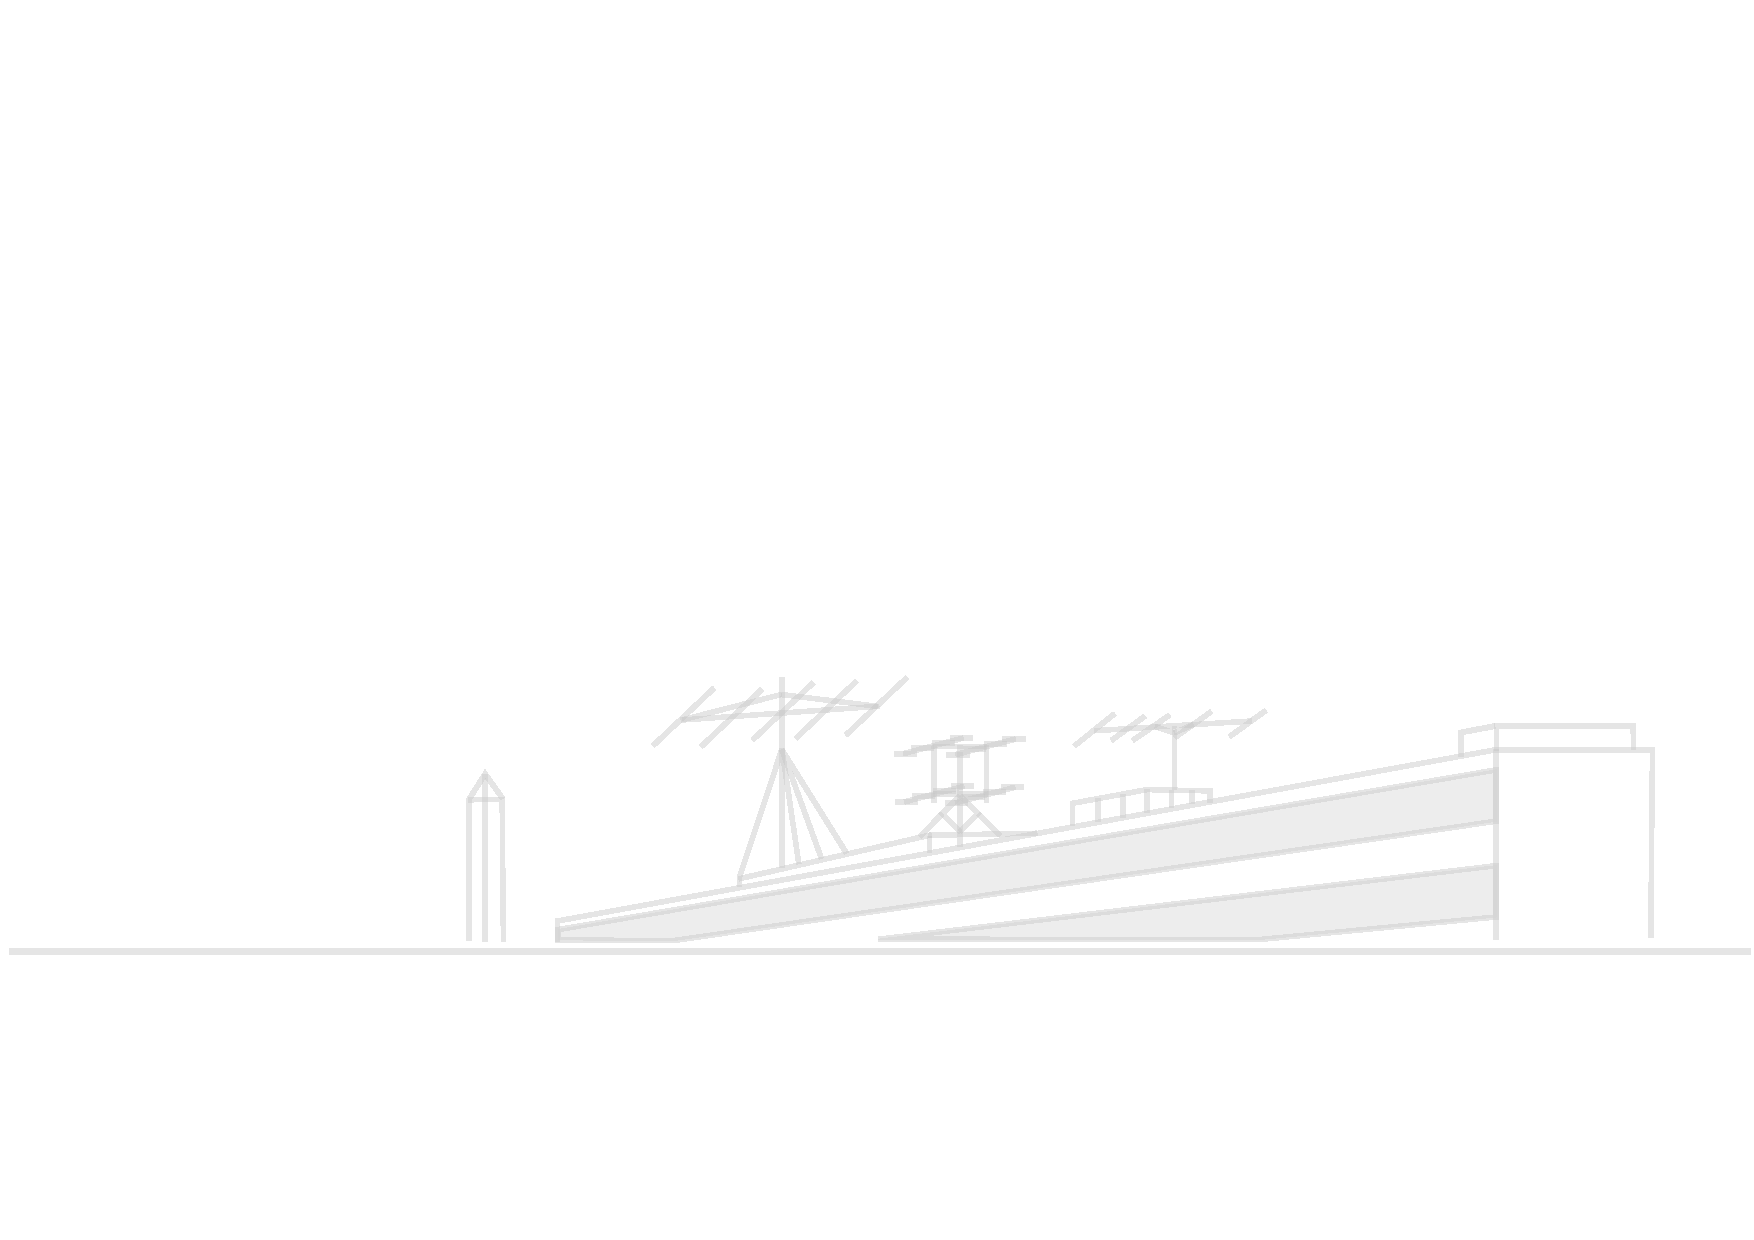
\includegraphics[width=17.8cm]{texdata/dk0tu_rooftop_background.pdf}
}

% Foliennummer einfügen
\setbeamertemplate{footline}[frame number]
%\setbeamertemplate{footline}{}

% Ändere das Zeichen vor jedem item
%\setbeamertemplate{itemize item}{\color{craneorange}$\blacktriangleright$}
%\setbeamertemplate{itemize subitem}{\color{craneorange}$\triangleright$}
%\setbeamertemplate{itemize subsubitem}{\color{craneorange}$\blacktriangleright$}

% Ändert die Blöcke 
\setbeamertemplate{blocks}[rounded][shadow=true]
% default | rounded [shadow=true|false]

%
% Eigene Kommandos
%

% Hack to get natbib and beamer working together. "The beamer user guide suggests
% that only the manual bibliography entry approach is supported"
% on some system it works out of the box, sometimes you need the hack :-(
% so check it --dl7bst
\ifdefined\newblock
    \relax
\else
    \newcommand{\newblock}{}
\fi

% \includedia command to generate png out of a dia file
% NEEDS installed dia and pdflatex option --shell-escape
\newcommand{\includedia}[1]{
    \immediate\write18{/usr/bin/dia #1.dia -e #1_diatmp.png -t png}
}

% RICHIG GROSSER FONT!
\newfont{\bigfont}{cmr10 at 144pt}
\newfont{\smallfont}{cmr10 at 8pt}

% Römische Ziffern
\makeatletter
\newcommand{\rmnum}[1]{\romannumeral #1}
\newcommand{\Rmnum}[1]{\expandafter\@slowromancap\romannumeral #1@}
\makeatother

% Schwarze Überschrift
%\setbeamercolor{frametitle}{fg=black}
%\setbeamercolor{title}{fg=black}

% Item- und Box-Farben
\definecolor{deepBlue}{HTML}{000066}
\setbeamercolor{itemize item}{fg=deepBlue}
\setbeamercolor{itemize subitem}{fg=deepBlue}
\setbeamercolor{description item}{fg=deepBlue}
\setbeamercolor{block title}{fg=deepBlue!100, bg=blue!15}
\setbeamercolor{block body}{fg=black, bg=blue!5}
\setbeamercolor{block title alerted}{fg=deepBlue, bg=red!75}
\setbeamercolor{block body alerted}{fg=black, bg=red!15}
\setbeamercolor*{block title example}{fg=blue!50, bg=blue!10}
\setbeamercolor*{block body example}{fg= blue, bg=blue!5}

%\setbeamercolor{section in head/foot}{parent=palette primary}
%\setbeamercolor{subsection in head/foot}{parent=palette secondary}
%\setbeamercolor{sidebar}{fg=darkblue,bg=yellow!90!orange}
%\setbeamercolor{title in sidebar}{fg=darkblue}
%\setbeamercolor{author in sidebar}{fg=darkblue}
%\setbeamercolor{section in sidebar}{fg=darkblue!10!black}
%\setbeamercolor{subsection in sidebar}{fg=darkblue!50!black}

% Titlepage Infos
\title{AFu-Kurs nach DJ4UF}
\author[DKØTU]{DKØTU\\ \footnotesize{Amateurfunkgruppe der TU Berlin}}
\institute[DKØTU]{\url{http://www.dk0tu.de} }

% PDF-Eigenschaften
\subject{DK0TU-Amateurfunkkurs nach DJ4UF}
\keywords{Amateurfunk Kurs HAM Radio Course CC-BY-NC-SA OpenSource TU Berlin DK0TU}

\subtitle{Technik Klasse E 04: \\
  Der Widerstand und seine Schaltungsarten \\[2em]}
\date{Stand 18.09.2017}
 \begin{document}

\begin{frame}
    \titlepage
    \vfill
    \begin{center}
        \ccbyncsaeu\\
        {\tiny This work is licensed under the \em{Creative Commons Attribution-NonCommercial-ShareAlike 3.0 License}.}\\[0.5ex]
         \tiny Amateurfunkgruppe der Technische Universität Berlin (AfuTUB), DKØTU
         %\includegraphics[scale=0.5]{img/DK0TU_Logo.pdf}
    \end{center}
\end{frame}


\section*{Einleitung}
\subsection*{Widerstand}

\begin{frame}
  \frametitle{Widerstand}
  \begin{center}
    \Large{Was ist das?} \\
    \Large{Wie sieht er aus?}
  \end{center}
\end{frame}


\begin{frame}
  \frametitle{Bauelement}

  \begin{center}
    \begin{figure}
      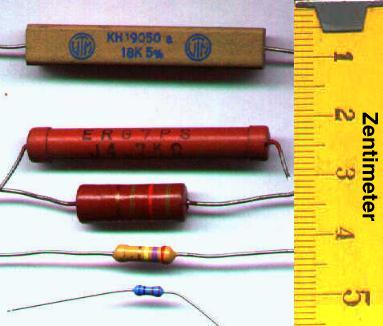
\includegraphics[width=1\textwidth,height=.75\textheight,keepaspectratio]{e04/Widerstaende.jpg}
      \caption{Drahtwiderstände \cite{wdst}}
      \label{fig_wdst}
      %\attribcaption{Widerstände}{Honina}{https://commons.wikimedia.org/wiki/File:Widerstände.JPG}{\ccbysa}
    \end{figure}
  \end{center}


\end{frame}

\begin{frame}
  \frametitle{Schaltbild}

  \begin{center}
    \begin{figure}
      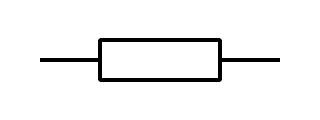
\includegraphics[width=.3\textwidth,height=.3\textheight,keepaspectratio]{e04/Resistor_symbol_IEC.png}
      \caption{Schaltsymbol nach IEC \cite{wdst_iec}}
      \label{fig_wdst_iec}
      %\attribcaption{Widerstandssymbol nach IEC}{Markus Kuhn}{https://commons.wikimedia.org/wiki/File:Resistor_symbol_IEC.svg}{\ccpd}
    \end{figure}
  \end{center}

  \begin{center}
    \begin{figure}
      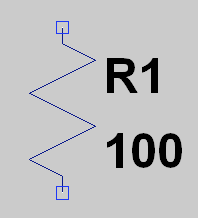
\includegraphics[width=.4\textwidth,height=.4\textheight,keepaspectratio]{e04/R_LTspice.png}
      %\caption{aus LTspice, Freeware zur Schaltungssimulation %\ExternalLink~\url{http://www.linear.com/designtools/software/\#Spice}}
    \end{figure}
  \end{center}

\end{frame}


\section*{Spezifischer Widerstand}

\begin{frame}
  \frametitle{Leitende Materialien}
  \begin{columns}
    \column{.6\textwidth}
    \begin{tabular}{lr}
      Material & Spezifischer Widerstand\footnotemark $\rho$ \\
        & $\text{ in } \frac{\Omega\cdot mm^2}{m}$ \\ \hline
      Silber & $1,587 \cdot 10^{-2}$ \\
      Kupfer & $1,721 \cdot 10^{-2}$ \\
      Gold & $2,214 \cdot 10^{-2}$ \\
      Aluminium & $2,65 \cdot 10^{-2}$ \\
      Zinn & $1,15 \cdot 10^{-1}$ \\
      Blei & $2,08 \cdot 10^{-1}$ \\
      Quecksilber & $9,412 \cdot 10^{-1}$ \\
      Germanium & \only<2>{$\leftarrow$ merken \hspace{2pc}} $4,6 \cdot 10^{5}$\\
      Porzellan & \only<2>{$\leftarrow$ \textbf{Isolator} \hspace{2pc}} $1 \cdot 10^{18}$ \\
    \end{tabular}

    \column{.35\textwidth}
    \only<3>{
    \begin{block}{Berechnung des Widerstands}
      $$R = \rho \cdot \frac{\ell}{A}$$
    \end{block}
    }
  \end{columns}
  \footnotetext[1]{\tiny \ExternalLink \url{http://de.wikipedia.org/wiki/Spezifischer_Widerstand}}
\end{frame}

\section*{Wider\-stands\-werte}

\begin{frame}
  \begin{center}
    \begin{figure}
      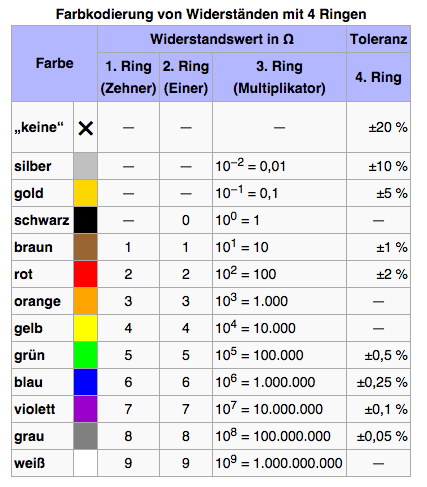
\includegraphics[width=\textwidth,height=.9\textheight,keepaspectratio]{e04/4-Ringe.png}
      \caption{Farbcodierung von Widerständen mit 4 Ringen \cite{ringe4}}
      \label{fig_ringe4}
      %\attribcaption{Farbkodierung von Widerständen mit 4 Ringen}{Screenshot}{https://de.wikipedia.org/wiki/Widerstand_(Bauelement)}{\ccbysa}
    \end{figure}
  \end{center}
\end{frame}

\begin{frame}
  \begin{center}
    \begin{figure}
      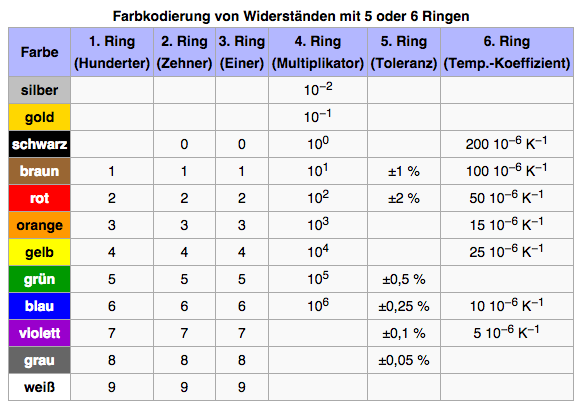
\includegraphics[width=\textwidth,height=.9\textheight,keepaspectratio]{e04/5-Ringe.png}
      \caption{Farbcodierung von Widerständen mit 5 Ringen \cite{ringe5}}
      \label{fig_ringe5}
      %\attribcaption{Farbkodierung von Widerständen mit 5 Ringen}{Screenshot}{https://de.wikipedia.org/wiki/Widerstand_(Bauelement)}{\ccbysa}
    \end{figure}
  \end{center}
\end{frame}

\begin{frame}
  \frametitle{SMD Widerstände}
  \begin{center}
    \begin{figure}
      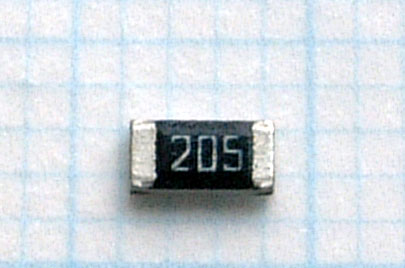
\includegraphics[width=\textwidth,height=.2\textheight,keepaspectratio]{e04/Rsistor_SMD.jpg}
      \caption{SMD-Widerstand \cite{smd}}
      \label{fig_smd}
      %\attribcaption{SMD Widerstand}{Haragayato}{https://commons.wikimedia.org/wiki/File:Register3.jpg}{\ccbysa}
    \end{figure}
  \end{center}

  \begin{center}
    \begin{tabular}{l||l|l|l|l|l|l|l|l|l|l}\hline
      1.Ziffer & - & 1 &2 & 3 & 4 & 5 & 6 & 7 & 8 & 9 \\ \hline
      2.Ziffer & 0 & 1 &2 & 3 & 4 & 5 & 6 & 7 & 8 & 9 \\ \hline
      3.Ziffer & 0 & 1 &2 & 3 & 4 & 5 & 6 & 7 &  &  \\ \hline
    \end{tabular}
  \end{center}
  \pause
  \begin{exampleblock}{Beispiel}
    \scriptsize
    \begin{center}
      \begin{tabular}{l|l}
        Aufdruck & Widerstandswert \\ \hline
        470 & $47 \cdot 10^{0} \Omega$ \\
        223 & $22 \cdot 10^{3} \Omega$ \\
        4R7 & $4,7 \Omega$ \\
      \end{tabular}
    \end{center}
  \end{exampleblock}

\end{frame}

\section*{Besondere Widerstandsarten}
\begin{frame}
  \frametitle{Potentiometer}

  \begin{center}
    \begin{figure}
      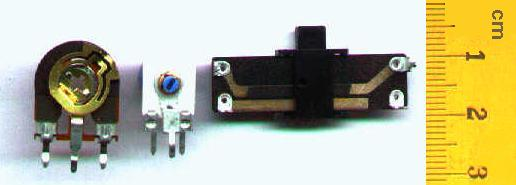
\includegraphics[width=\textwidth,height=.75\textheight,keepaspectratio]{e04/Potenziometer.jpg}
      \caption{Potentiometer \cite{potentiometer}}
      \label{fig_potentiometer}
      %\attribcaption{Zwei Trimmpotentiometer und ein Schiebepotentiometer}{Honina}{https://commons.wikimedia.org/wiki/File:Potenziometer.JPG}{\ccbysa}
    \end{figure}
  \end{center}

\end{frame}

\begin{frame}
  \frametitle{Besondere Widerstände}

  \begin{center}
    \begin{figure}
      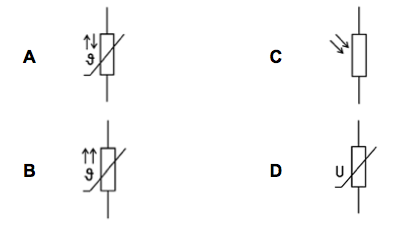
\includegraphics[width=.6\textwidth,height=.5\textheight,keepaspectratio]{e04/bild-TC106.png}
      \caption{Technik Fragenkatalog Klasse E 2006-09 Frage TC106}
    \end{figure}

    \begin{tabular}{l||l}\hline
      A & NTC - Negativer Temperaturkoeffizient \\ \hline
      B & PTC - Positiver Temperaturkoeffizient \\ \hline
      C & Lichteinfallgesteuerter Widerstand (Lichtsensor) \\ \hline
      D & Spannungsgesteuerter Widerstand \\ \hline
    \end{tabular}
  \end{center}
\end{frame}


\section*{Schaltungen}

\begin{frame}
  \frametitle{Reihenschaltung}

  \begin{columns}
    \column{.4\textwidth}
    \begin{center}
      \begin{figure}
        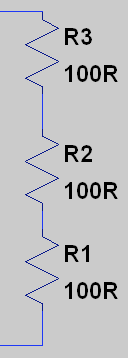
\includegraphics[width=.4\textwidth,height=.75\textheight,keepaspectratio]{e04/Reihe.png}
        \caption{aus LTspice}
      \end{figure}
    \end{center}
    \pause
    \column{.55\textwidth}
    \begin{block}{Berechnung}
      $$R_{gesamt} = R_1 + R_2 + R_3 + ...$$
    \end{block}
  \end{columns}

\end{frame}

\begin{frame}
  \frametitle{Parallelschaltung}
  \begin{columns}
    \column{.4\textwidth}
    \begin{center}
      \begin{figure}
        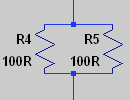
\includegraphics[width=\textwidth,height=.75\textheight,keepaspectratio]{e04/Parallel.png}
        \caption{aus LTspice}
      \end{figure}
    \end{center}
    \pause
    \column{.55\textwidth}
    \begin{block}{Berechnung}
      $$\frac{1}{R_{gesamt}} = \frac{1}{R_1} + \frac{1}{R_2} + \frac{1}{R_3} + ...$$
    \end{block}
  \end{columns}
\end{frame}

\begin{frame}
  \frametitle{Ersatzwiderstand}
  \begin{columns}
    \column{.47\textwidth}
    \begin{figure}
      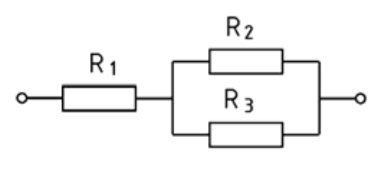
\includegraphics[width=.75\textwidth,height=.3\textheight,keepaspectratio]{e04/Ersatzwiderstand1.png}
      \caption{aus dem Fragenkatalog}
    \end{figure}
    \column{.47\textwidth}
    \begin{figure}
      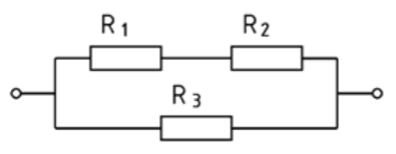
\includegraphics[width=.75\textwidth,height=.3\textheight,keepaspectratio]{e04/Ersatzwiderstand2.png}
      \caption{aus dem Fragenkatalog}
    \end{figure}
  \end{columns}
  \begin{columns}
    \column{.47\textwidth}
    \pause
    \begin{exampleblock}{Berechnung}
      $R_1 + (R_2 \parallel R_3)$ \\[1.5em]
      $\Rightarrow R_1 + \cfrac{1}{\cfrac{1}{R_2} + \cfrac{1}{R_3}}$
    \end{exampleblock}
    \column{.47\textwidth}
    \pause
    \begin{exampleblock}{Berechnung}
      $(R_1 + R_2) \parallel R_3$\\[1.5em]
      $\Rightarrow \cfrac{1}{\cfrac{1}{R_1 + R_2} + \cfrac{1}{R_3}}$
    \end{exampleblock}
  \end{columns}
\end{frame}

\begin{frame}
  \frametitle{Spannungsteiler}
  \begin{columns}
    \column{.4\textwidth}
    \begin{center}
      \begin{figure}
        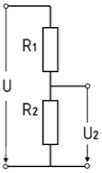
\includegraphics[width=.6\textwidth,height=.75\textheight,keepaspectratio]{e04/Spannungsteiler.png}
        \caption{aus dem Fragenkatalog}
      \end{figure}
    \end{center}
    \column{.55\textwidth}
    \begin{block}{Berechnung}
      $\cfrac{U}{R_1 + R_2} = \cfrac{U_2}{R_2} = \cfrac{U_1}{R_1}$
    \end{block}
  \end{columns}
\end{frame}

\begin{frame}
	\frametitle{Stromteiler}
	\begin{columns}
		\column{.4\textwidth}
		\begin{center}
			\begin{figure}
				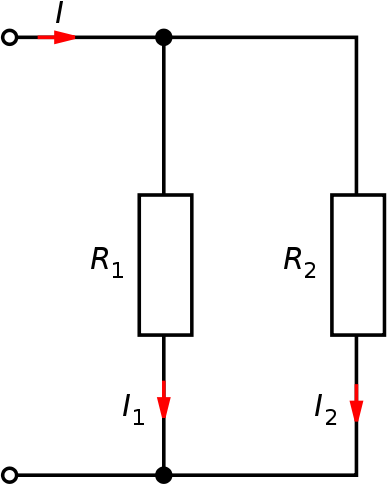
\includegraphics[width=.6\textwidth,height=.75\textheight,keepaspectratio]{e04/Stromteiler.png}
				\caption{Stromteiler \cite{stromteiler}}
				\label{fig_stromteiler}
			\end{figure}
		\end{center}
		\column{.55\textwidth}
		\begin{block}{Berechnung}
			$\cfrac{I_1}{I_2} = \cfrac{R_2}{R_1}$
		\end{block}
	\end{columns}
\end{frame}

%\begin{frame}
%  \begin{alertblock}{Hausaufgabe}
%    Aus Fragenkatalog Klasse E Kapitel 1.3.1 ``Widerstand'' (TC101--TC111) durcharbeiten.\\
%    Aus Fragenkatalog Klasse E Kapitel TD101--TD104, TD108--TD110 berechnen.
%  \end{alertblock}
%\end{frame}

\section*{Übungen}

\begin{frame}
  \frametitle{Übungen}
%  \pause
  \begin{center}
    Einführung Steckbrett
  \end{center}
\end{frame}

%\subsection*{Übung 1}
%\begin{frame}
%  \begin{columns}
%    \column{0.4\textwidth}
%    \begin{center}
%      \begin{figure}
%        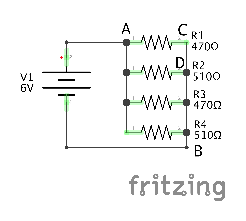
\includegraphics[width=1\textwidth]{e04/Uebung1_Schaltplan.pdf}
%      \end{figure}
%    \end{center}
%    \column{0.55\textwidth}
%    \begin{alertblock}{Aufgabe 1}
%      Baue die Schaltung auf dem Steckbrett auf.\\
%      Berechne den Ersatzwiderstand. Miss zur Überprüfung den Gesamtwiderstand.
%    \end{alertblock}
%    \begin{alertblock}{Aufgabe 2}
%      Berechne die Spannung über $R_1$, $R_2$, $R_3$ und $R_4$. Miss zur Überprüfung nach.\\
%      Miss und erkläre die Spannungen über $A$---$B$, $A$---$C$ und $A$---$D$.
%    \end{alertblock}
%  \end{columns}
%  \begin{alertblock}{Aufgabe 3}
%    Berechne die Ströme durch $R_1$, $R_2$, $R_3$, $R_4$ und den Gesamtstrom. Miss zur %Überprüfung nach.
%  \end{alertblock}
%\end{frame}

%\subsection*{Übung 2}
%\begin{frame}
%  \begin{columns}
%    \column{0.4\textwidth}
%    \begin{center}
%      \begin{figure}
%        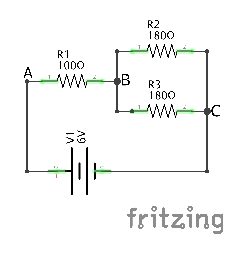
\includegraphics[width=1\textwidth]{e04/Uebung2_Schaltplan.pdf}
%      \end{figure}
%    \end{center}
%    \column{0.55\textwidth}
%    \begin{alertblock}{Aufgabe 1}
%      Baue die Schaltung auf dem Steckbrett auf.
%      Berechne den Ersatzwiderstand. Miss zur Überprüfung den Gesamtwiderstand.
%    \end{alertblock}
%    \begin{alertblock}{Aufgabe 2}
%      Berechne die Spannung über $R_1$, $R_2$ und $R_3$. Miss zur Überprüfung nach.\\
%      Miss und erkläre die Spannungen über $A$---$B$, $A$---$C$ und $B$---$C$.
%    \end{alertblock}
%  \end{columns}
%  \begin{alertblock}{Aufgabe 3}
%    Berechne die Ströme durch $R_1$, $R_2$, $R_3$ und den Gesamtstrom. Miss zur Überprüfung %nach.
%  \end{alertblock}
%\end{frame}

\subsection*{Übung 3}
\begin{frame}
  \begin{alertblock}{Zusatzaufgabe}
    Die rote Leuchtdiode benötigt einen Strom von $20mA$. Für die Aufgabe sei erstmal angenommen, dass keine Spannung über die Leuchtdiode abfällt. Dimensioniere einen Spannungsteiler so, dass mit der gegebenen Batterie von 6V an der Leuchtdiode eine Spannung von 3V bis 5V anliegt. Gegeben sind die Widerstände in der Größe $4\times100\Omega$, $2\times180\Omega$, $4\times470\Omega$ und $2\times510\Omega$. Berechne zuerst den Spannungsteiler und zeichne einen Schaltplan.
  \end{alertblock}
%  \begin{alertblock}{Aufgabe 2}
%    Baue die Schaltung auf. Die abgeflachte Seite der Leuchtdiode zeigt zu Minus. Miss den %Strom durch die Leuchtdiode. Miss die Spannung über die Widerstände. Wie lautet die %Gesamtsumme der Spannungen über die Widerstände? Erkläre.
%  \end{alertblock}
%  \begin{alertblock}{Aufgabe 3}
%    Die Leuchtdiode soll dunkler leuchten. Muss dazu mehr oder weniger Strom fließen? Wie %sind die Widerstände zu dimensionieren?
%  \end{alertblock}
\end{frame}


\section*{Referenzen}

\begin{frame}
  \frametitle{Referenzen/Links}

  \footnotesize
  \begin{itemize}
    \item Moltrecht E 04: \\
      \url{https://www.darc.de/der-club/referate/ajw/lehrgang-te/e04/}
      
    \bibitem{wdst}  Abbildung \ref{fig_wdst}: Drahtwiderstände\\
	    \url{https://commons.wikimedia.org/wiki/File:Widerstande.JPG}\\
	\bibitem{wdst_iec}  Abbildung \ref{fig_wdst_iec}: Schaltsymbol nach IEC\\
		\url{https://commons.wikimedia.org/wiki/File:Resistor\_symbol\_IEC.svg}\\
    \bibitem{ringe4}  Abbildung \ref{fig_ringe4}: Farbcodierungstafel\\
		\url{https://de.wikipedia.org/wiki/Widerstand\_(Bauelement)}\\
	\bibitem{ringe5}  Abbildung \ref{fig_ringe5}: Farbcodierungstafel\\
		\url{https://de.wikipedia.org/wiki/Widerstand\_(Bauelement)}\\
    \bibitem{smd}  Abbildung \ref{fig_smd}: SMD-Widerstand\\
		\url{https://commons.wikimedia.org/wiki/File:Register3.jpg}\\
	\bibitem{potentiometer}  Abbildung \ref{fig_potentiometer}: Potentiometer\\
		\url{https://commons.wikimedia.org/wiki/File:Potenziometer.JPG}\\
	\bibitem{stromteiler}  Abbildung \ref{fig_stromteiler}: Stromteiler\\
		\url{https://commons.wikimedia.org/wiki/File:Stromteiler.svg}\\

  \end{itemize}

\end{frame}

% Hier könnte noch eine Kontaktfolie stehen

\end{document}

